%!TEX root =  ../main.tex

\subsection{Numerically}

\objective{Calculate and graph reciprocal functions.}

Calculating the reciprocal of a function is very straightforward.  For any given $x$,
take the output $f(x)$, and then reciprocate that number.  What that leads to is a
complicated picture.  However, a pattern emerges.  The reciprocal of 1 is 1, and the
reciprocal of -1 is -1.  That means points on the graph with a $y$ of 1 will not
be effected by reciprocation.  Other integer outputs will reciprocate to smaller and
smaller fractions, e.g. 2 to $\frac{1}{2}$, 3 to $\frac{1}{3}$, etc.

What is unusual is the behavior around 0.  Zero has no reciprocal, so there will 
typically be a vertical asymptote.

Especially in trigonometry, reciprocals can have names.

\begin{figure}
\begin{centering}
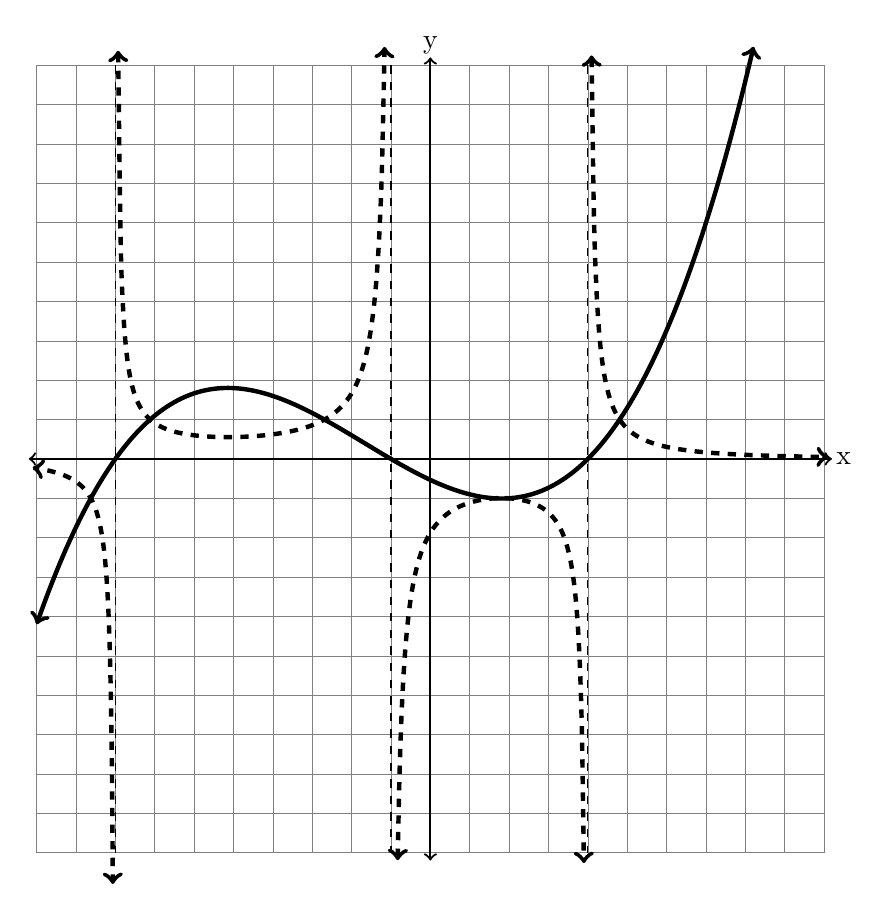
\begin{tikzpicture}[scale=0.5]
	\draw [help lines] (-10, -10) grid (10, 10);
	\draw [thick,<->] (-10.2, 0) -- (10.2, 0);
	\draw [thick,<->] (0, -10.2) -- (0, 10.2);
        % x-axis label
        \node at (10.5, 0) {x};
        % y-axis label
        \node at (0, 10.5) {y};
        \draw[domain=-10:8.21,<->,ultra thick,samples=100,smooth] plot (\x,{1/60*(\x-4)*(\x+1)*(\x+8)});
        \draw[domain=-10.1:-8.065,<->,ultra thick,samples=100,smooth,dashed] plot (\x,{60/((\x-4)*(\x+1)*(\x+8))});
        \draw[domain=-7.93:-1.162,<->,ultra thick,samples=100,smooth,dashed] plot (\x,{60/((\x-4)*(\x+1)*(\x+8))});
        \draw[domain=-.83:3.9,<->,ultra thick,samples=100,smooth,dashed] plot (\x,{60/((\x-4)*(\x+1)*(\x+8))});
        \draw[domain=4.095:10.1,<->,ultra thick,samples=100,smooth,dashed] plot (\x,{60/((\x-4)*(\x+1)*(\x+8))});
        \draw[dashed, -] (-1,10) -- (-1,-10);
        \draw[dashed, -] (-8,10) -- (-8,-10);
        \draw[dashed, -] (4,10) -- (4,-10);
\end{tikzpicture}
\caption[Example of graphical reciprocation]{An example of a function and its reciprocal, $f(x)=\frac{1}{60}(x-4)(x+1)(x+8)$.}
\end{centering}
\end{figure}